%% --------------------------------------------------------------------
%% Template UTEC Tesis - Estructura Oficial PFC
%% --------------------------------------------------------------------
\documentclass[a4paper,12pt,oneside]{tesisutec}

\selectlanguage{spanish}

%% Paquetes
\usepackage[utf8]{inputenc}
\usepackage[square, numbers, comma, sort&compress]{natbib}
\usepackage[spanish]{babel}
\usepackage{float}
\usepackage[spanish,onelanguage,ruled,vlined]{algorithm2e}
\usepackage{verbatim} 
\usepackage{hyperref}
\usepackage{notoccite}

% Ubicación de las imágenes
\graphicspath{{images/}}

\makeatletter
\def\algbackskip{\hskip-\ALG@thistlm}
\makeatother

\hypersetup{urlcolor=blue, colorlinks=true}

\begin{document}

\frontmatter

\department{CIENCIAS DE LA COMPUTACIÓN}
\degree{Licenciado}
\major{Ciencias de la Computación}

\title{TÍTULO DEL TRABAJO DE INVESTIGACIÓN}

\author{
  Alejandro Gerardo Calizaya Álvarez \orcid{0000-0000-0000-0000}\\[0.2cm]
  Jerimy Pierre Sandoval Rivera \orcid{0000-0000-0000-0000}\\[0.2cm]
  César Aarón Perales Rosales \orcid{0000-0000-0000-0000}
}

\supervisor{
  Eric Biagioli \orcid{0000-0000-0000-0000}%\\[0.2cm]
  %Germain Garcia Zanabria \orcid{0000-0000-0000-0000}
}
\date{2026}

\maketitle

\setstretch{1.5}

\chapter*{Dedicatoria}
Para mi perrito, porque tiene mucha hambre.
\input{encabezados/agradecimientos}

\tableofcontents
\newpage
\listoftables
\newpage
\listoffigures

\addtocontents{toc}{\vspace{1.5em}}

%% ============================================================================
\mainmatter
\pagestyle{fancy}

\chapter*{Resumen}
\addcontentsline{toc}{chapter}{Resumen}

El análisis espacial de fenómenos urbanos, como la criminalidad, requiere la asignación precisa de eventos georreferenciados sobre la infraestructura vial mediante procesos de \textit{Map Matching}. Sin embargo, los grafos urbanos extraídos de fuentes de datos abiertas como OpenStreetMap presentan una densidad geométrica masiva que incrementa significativamente la complejidad temporal y espacial de las consultas geográficas. 

Este trabajo de investigación propone y evalúa algoritmos de simplificación topológica de redes urbanas orientados a optimizar la eficiencia computacional en la asignación de datos delictivos. Para ello, se diseña e implementa una arquitectura modular que incorpora un \textit{pipeline} de evaluación estandarizado. Este marco permite cuantificar rigurosamente el impacto de la reducción de nodos y aristas a través de métricas objetivas, tales como el ratio de compresión topológica y la invarianza en la longitud de aristas. 

La solución computacional integra estructuras de indexación espacial avanzadas para acelerar las proyecciones geométricas en coordenadas planas. Los resultados obtenidos demuestran que es factible reducir drásticamente la huella de memoria del grafo y los tiempos de procesamiento de consultas espaciales, sin comprometer la precisión geométrica de la asignación ni alterar las invariantes topológicas necesarias para el análisis espacial urbano a gran escala.

\vspace{1cm}
\noindent \textbf{Palabras clave:} \textit{Map Matching}, Simplificación de Grafos, OpenStreetMap, Análisis Espacial, Estructuras de Datos Espaciales, Redes Urbanas.



\chapter*{Abstract}
\addcontentsline{toc}{chapter}{Abstract}

The spatial analysis of urban phenomena, such as crime, relies on the accurate assignment of georeferenced events to road infrastructure through Map Matching processes. However, urban graphs extracted from open data sources like OpenStreetMap exhibit a massive geometric density that significantly increases the temporal and spatial complexity of geographic queries.

This research proposes and evaluates topological simplification algorithms for urban networks, aimed at optimizing computational efficiency in the spatial assignment of crime data. To achieve this, a modular architecture incorporating a standardized evaluation pipeline is designed and implemented. This framework allows for the rigorous quantification of the impact of node and edge reduction through objective metrics, such as the topological compression ratio and edge length invariance.

The computational solution integrates advanced spatial indexing structures to accelerate geometric projections in planar coordinates. The results demonstrate that it is feasible to drastically reduce the memory footprint of the graph and the processing times for spatial queries, without compromising the geometric accuracy of the assignment or altering the fundamental topological invariants required for large-scale urban spatial analysis.

\vspace{1cm}
\noindent \textbf{Keywords:} Map Matching, Graph Simplification, OpenStreetMap, Spatial Analysis, Spatial Data Structures, Urban Networks.

\chapter{Contexto y Definición del Problema}
% 

\section{Descripción clara del problema a ser resuelto}

Las ciudades modernas generan continuamente grandes cantidades de información georreferenciada como resultado de diversas actividades urbanas, incluyendo reportes de criminalidad, accidentes de tránsito, sistemas de transporte y plataformas digitales basadas en localización \cite{huang2021analytics, ramirez2021sensors, kamrowska2021impact}. El crecimiento sostenido de estas fuentes ha incrementado significativamente la disponibilidad de datos espaciales capaces de describir fenómenos que ocurren sobre el territorio urbano \cite{huang2021analytics, avram2026advancing}. Esta abundancia ha impulsado el desarrollo de metodologías de análisis geoespacial orientadas a comprender patrones espaciales y extraer conocimiento útil. Como consecuencia, el procesamiento eficiente de grandes volúmenes de información geográfica se ha convertido en un componente fundamental para apoyar la planificación urbana y la toma de decisiones basadas en evidencia \cite{huang2021analytics, kamrowska2021impact, avram2026advancing}.

En este contexto, el análisis espacial de eventos urbanos —como la incidencia criminal— exige identificar la ubicación exacta y la frecuencia de los sucesos para descubrir patrones territoriales. El estado del arte demuestra que este análisis se formaliza asignando las coordenadas de los eventos a un grafo espacial que modela la infraestructura vial, dado que las redes urbanas condicionan intrínsecamente la distribución de estos fenómenos \cite{kozhabek2025multi, yap2023urbanity}. Mediante procesos de \textit{Map Matching}, la información cruda se vincula a representaciones topológicas para su evaluación analítica \cite{xue2022quantifying}.

Sin embargo, los grafos urbanos extraídos directamente de bases de datos espaciales abiertas, como OpenStreetMap (OSM), sufren de una excesiva densidad geométrica. Estas redes presentan múltiples aristas paralelas y vértices con conexiones redundantes (necesarias para el trazado de mapas visuales) que no aportan información analítica funcional sobre el evento urbano.

Esta densidad genera un grave problema de \textbf{dilución o dispersión espacial}. Es decir, si se asigna un conjunto de eventos a un grafo crudo, la verdadera densidad del fenómeno se pierde al redistribuirse estadísticamente entre múltiples aristas adyacentes, en lugar de concentrarse en una única vía lógica. 

Como se ejemplifica en la Figura \ref{fig:dilucion_semantica}, al evaluar una avenida con múltiples carriles paralelos, los eventos delictivos pueden distribuirse entre diferentes elementos de la red aun cuando correspondan funcionalmente a una misma vía urbana. Esta situación puede dificultar la identificación de patrones espaciales consistentes y afectar la interpretación de indicadores de densidad o concentración. En consecuencia, surge la necesidad de explorar representaciones alternativas que permitan preservar la estructura vial relevante para el análisis sin introducir distorsiones significativas en la distribución espacial de los eventos.

\begin{figure}[H]
    \centering
    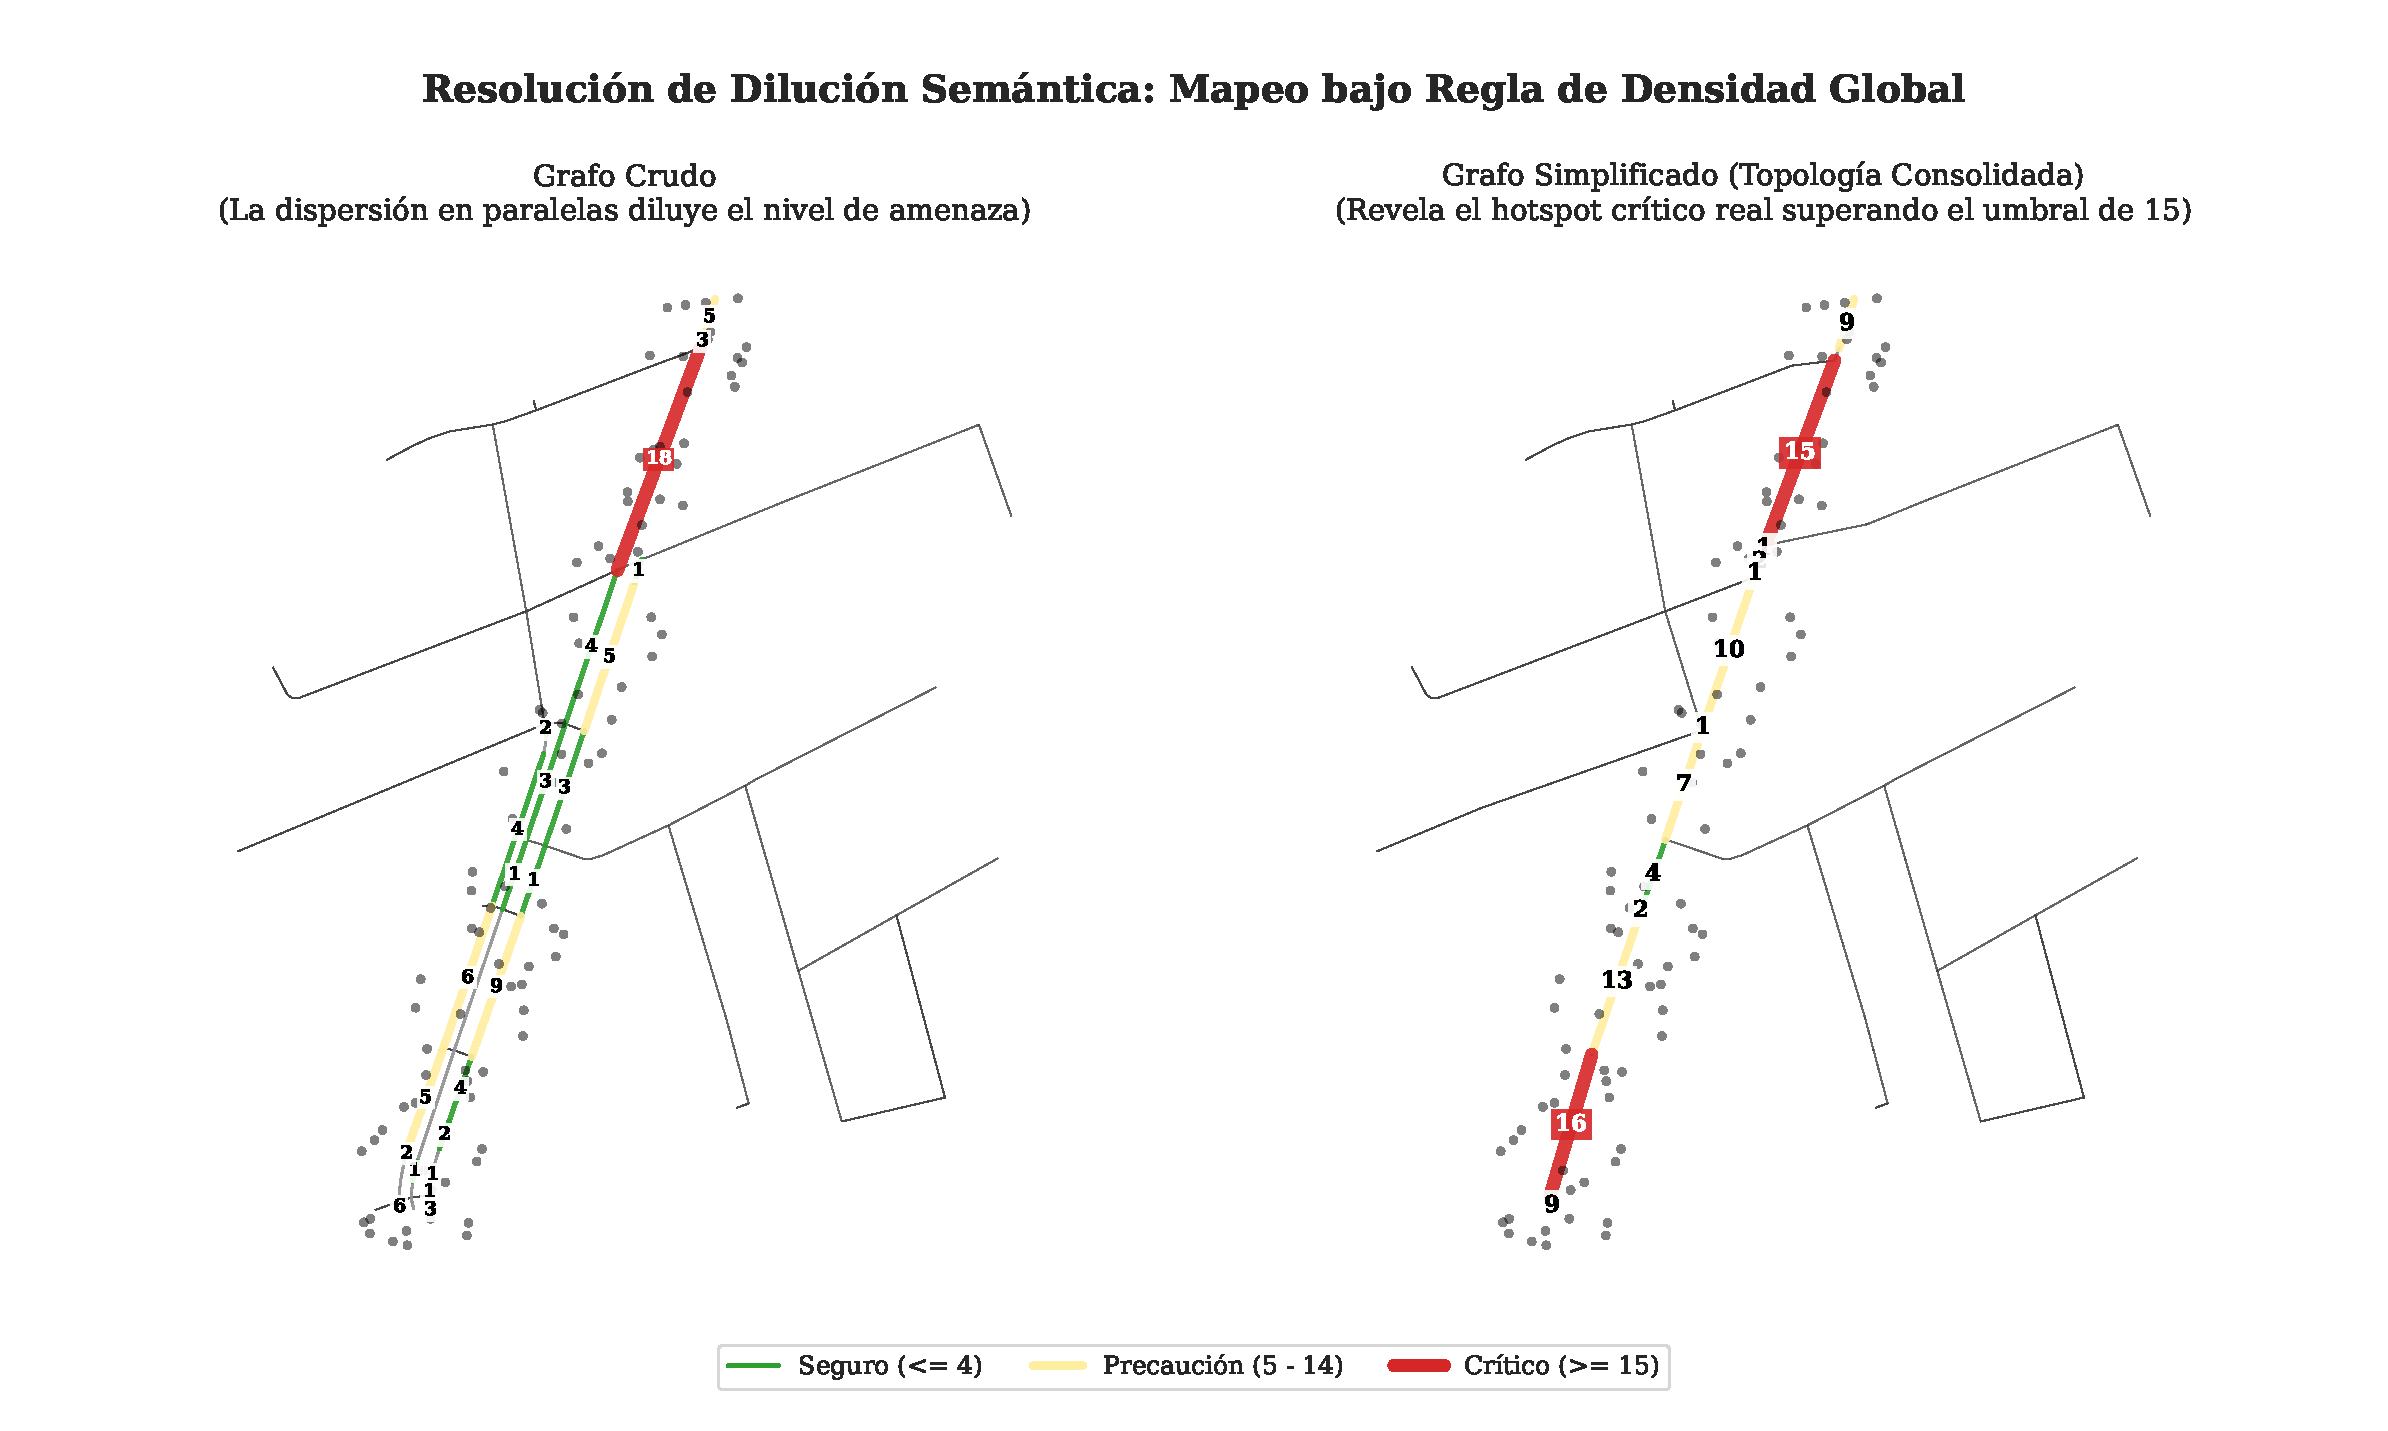
\includegraphics[
        width=\textwidth,
        trim=3.5cm 0cm 3.5cm 0cm,
        clip
    ]{../images/disolucion_semantica.pdf}
    \caption{Impacto de la granularidad topológica en el análisis de densidad espacial. A la izquierda, la red cruda diluye los eventos sobre aristas paralelas, ocultando la amenaza real. A la derecha, el colapso semántico del grafo concentra los eventos sobre la vía lógica, revelando la verdadera magnitud del \textit{hotspot}.}
    \label{fig:dilucion_semantica}
\end{figure}

Si bien existen diversos métodos de simplificación de redes urbanas, gran parte de ellos han sido diseñados con objetivos orientados a la compresión geométrica, la representación cartográfica o la reducción de complejidad estructural. Sin embargo, la influencia de estas transformaciones sobre la distribución espacial de eventos y sobre la preservación de propiedades analíticas relevantes continúa siendo un aspecto que requiere mayor investigación.

Por lo tanto, la pregunta de investigación central es: ¿Cómo simplificar eficientemente un grafo espacial urbano para concentrar la densidad de eventos, garantizando la recuperación de su semántica original sin alterar las invariantes topológicas que definen la ciudad?

\section{Motivación y relevancia (técnica, social, económica)}

La implementación de algoritmos avanzados de simplificación topológica se justifica bajo tres dimensiones fundamentales:

\begin{itemize}
    \item \textbf{Relevancia técnica:} Los algoritmos de ruteo y \textit{Map Matching} estándar sufren una severa sobrecarga de memoria y tiempo de procesamiento cuando operan sobre redes a escala de ciudad. La simplificación geométrica rigurosa proporciona ahorros significativos de memoria (RAM) al reducir la dimensionalidad del grafo $|V| + |E|$. Esto permite diseñar arquitecturas escalables donde las consultas espaciales operan con una rapidez drásticamente mayor, sin sacrificar la semántica analítica del sistema.
    
    \item \textbf{Relevancia social:} Prevenir la dilución espacial es crítico para la seguridad ciudadana. Un mapeo eficiente y concentrado permite a las autoridades identificar y predecir \textit{hotspots} criminales con alta fidelidad, optimizando el diseño de estrategias de prevención y la asignación de rutas de patrullaje.
    
    \item \textbf{Relevancia económica:} Al reducir el peso del modelo espacial y acelerar los tiempos de cómputo, se disminuyen radicalmente los ciclos de CPU y los requerimientos de infraestructura (\textit{Cloud Computing}), abaratando los costos operativos de despliegue para entidades gubernamentales o investigativas.
\end{itemize}

\section{Impacto esperado}

Se proyecta que la arquitectura propuesta genere dos impactos críticos en el análisis de redes urbanas:

\begin{enumerate}
    \item \textbf{Mejora en la eficiencia computacional:} Mediante la reducción de la complejidad estructural de la red y el uso de mecanismos eficientes de indexación espacial, se espera disminuir significativamente los tiempos requeridos para operaciones de asignación espacial y análisis sobre grandes volúmenes de eventos georreferenciados.
    
    \item \textbf{Preservación estricta de la topología y precisión:} La simplificación no debe entenderse como la destrucción de datos, sino como su consolidación. Se espera mantener el error de proyección espacial (bajo el estándar EPSG:3857) cercano a cero. Fundamentalmente, se busca conservar propiedades asociadas a conectividad, navegabilidad y consistencia de rutas, de manera que la red simplificada continúe siendo útil para aplicaciones de análisis espacial.
\end{enumerate}

\section{Formulación de suposiciones e identificación de restricciones}

Para delimitar el alcance del presente trabajo, se establecen las siguientes suposiciones:
\begin{itemize}
    \item Los datos delictivos son entidades discretas y estáticas representadas por coordenadas geográficas bidimensionales.
    
    \item OpenStreetMap (OSM) será utilizado como fuente cartográfica de referencia debido a su amplia adopción en investigaciones de análisis espacial, movilidad urbana y redes de transporte.

    \item \textbf{Inferencia Semántica:} Se asume que la semántica topológica de una red urbana no puede inferirse puramente a través de métodos geométricos abstractos (como distancias euclidianas). Para una simplificación correcta, es imperativo \textit{recuperar} la semántica inyectando información auxiliar extraída del dominio del grafo (tales como nombres de vías, tipos de \textit{highway} y jerarquía de conexión).
\end{itemize}

Asimismo, se identifican las siguientes restricciones en el diseño experimental:
\begin{itemize}
    \item El análisis se efectuará sobre un modelo de red estático, excluyendo variables de fricción dinámica como velocidades en tiempo real o densidades de tráfico fluctuantes.
    \item El alcance computacional se concentra exclusivamente en las fases de preprocesamiento, simplificación topológica estructurada y la asignación espacial de puntos estáticos.
\end{itemize} %%
\chapter{Fundamentos Teóricos}

El presente capítulo expone el marco teórico y matemático que sustenta las dos contribuciones principales de esta investigación: la ingestión espacial eficiente de datos masivos y el desarrollo de un algoritmo de simplificación adaptativa para redes viales urbanas. Inicialmente, se formalizan las redes de transporte desde la perspectiva de la teoría de grafos y la geometría computacional. Posteriormente, se abordan los fundamentos de la asignación espacial y las estructuras de indexación geométrica las cuales constituyen el núcleo teórico para la carga rápida de bases de datos espaciales. Finalmente, se analizan los algoritmos de generalización de líneas y se deducen formalmente las métricas de invarianza estructural empleadas para evaluar la calidad topológica de la red resultante.

% =====================================================================
\section{Teoría de Grafos y Redes Espaciales Urbanas}
% =====================================================================

El modelado computacional de la infraestructura vial de una ciudad requiere abstraer elementos físicos continuos como avenidas, calles y autopistas en estructuras de datos discretas que permitan el análisis de rutas y la gestión de bases de datos geoespaciales. Esta sección introduce la formalización abstracta de las redes urbanas y detalla las restricciones geométricas y topológicas implícitas en los sistemas viales modernos.

\subsection{Formalización del Grafo Vial Embebido}

Para comprender la complejidad de las redes viales, es necesario establecer la distinción fundamental entre un grafo abstracto o tradicional y un grafo espacialmente embebido en el plano.

Un grafo abstracto se define formalmente como un par ordenado $G = (V, E)$, donde $V$ es un conjunto finito de vértices o nodos, y $E \subseteq V \times V$ es un conjunto de aristas que representan relaciones binarias lógicas entre dichos nodos. En este tipo de estructura de datos pura, el interés radica únicamente en la conectividad. Conceptos como la distancia métrica, la curvatura, la orientación o la posición geográfica no existen en la definición formal de un grafo abstracto.

Por el contrario, un grafo espacialmente embebido es una estructura donde la conectividad lógica está intrínsecamente ligada a un espacio geométrico continuo, típicamente el plano euclidiano $\mathbb{R}^2$. En el contexto vial, este formalismo se expande mediante dos funciones de mapeo esenciales:

\begin{enumerate}
    \item \textbf{Mapeo de Vértices ($\mathcal{C}$):} Asigna a cada nodo una posición espacial explícita mediante un vector de coordenadas cartesianas proyectadas:
    \begin{equation}
    \mathcal{C}: V \rightarrow \mathbb{R}^2 \quad \text{donde} \quad \mathcal{C}(v_i) = (x_i, y_i)
    \end{equation}
    
    \item \textbf{Mapeo de Aristas ($\mathcal{G}$):} A diferencia de un grafo abstracto donde una arista es un par ordenado ideal, en una red espacial cada arista $e \in E$ está ligada a un soporte geométrico continuo conocido como polyline o LineString. Este soporte se define como una secuencia ordenada de $k$ puntos de forma en el plano:
    \begin{equation}
    \mathcal{G}(e) = \langle p_1, p_2, \dots, p_k \rangle \quad \text{con} \quad p_m \in \mathbb{R}^2
    \end{equation}
    donde el primer punto $p_1$ coincide con la posición del nodo origen $\mathcal{C}(v_i)$ y el último punto $p_k$ corresponde al nodo destino $\mathcal{C}(v_j)$.
\end{enumerate}

Adicionalmente, los grafos lineales puros asumen una propiedad de planariedad estricta, es decir, donde dos aristas no pueden cruzarse en el plano sin intersectar sus vértices. Sin embargo, las redes viales reales se catalogan como grafos espaciales no-planares. La presencia de infraestructuras multinivel, tales como puentes elevados, pasos a desnivel y túneles, implica la existencia de aristas cuyos soportes geométricos $\mathcal{G}(e_1)$ y $\mathcal{G}(e_2)$ se cruzan en la proyección bidimensional $\mathbb{R}^2$ pero no comparten un nodo real de articulación vial en el espacio tridimensional.

Para capturar con total fidelidad el comportamiento del tránsito vehicular y la morfología urbana, un grafo embebido simple resulta insuficiente. Esta investigación formaliza la red urbana como un \textbf{Multigrafo Dirigido Espacial} (Spatial MultiDiGraph). La elección de este modelo matemático específico responde a dos variables críticas:

\begin{itemize}
    \item \textbf{Direccionalidad (Grafo Dirigido):} El flujo vehicular está restringido por leyes de tránsito. Si una vía es de un solo sentido, la arista posee una orientación estricta $(v_i, v_j)$. Si la vía es de doble sentido, se modela mediante dos aristas independientes con orientaciones opuestas: $e_1 = (v_i, v_j)$ y $e_2 = (v_j, v_i)$.
    \item \textbf{Multiplicidad (Multigrafo):} Existen escenarios urbanos donde dos intersecciones contiguas están conectadas por más de una infraestructura vial independiente (por ejemplo, una calzada central expresa y una calzada lateral de servicio que corren en paralelo). Un multigrafo permite la existencia de aristas paralelas compartiendo los mismos nodos extremos, diferenciándose mediante un identificador único (\textit{edge id}).
\end{itemize}

Formalmente, el Multigrafo Dirigido Espacial se define mediante la tupla:

\begin{equation}
G = (V, E, \Psi, \mathcal{C}, \mathcal{G})
\end{equation}

Donde $V$ es el conjunto de intersecciones, $E$ es el conjunto de segmentos viales, y $\Psi: E \rightarrow V \times V \times \mathbb{N}$ es una función de incidencia que asocia cada arista a un par ordenado de vértices junto con un índice único que resuelve la multiplicidad. 

Finalmente, para asegurar que los cálculos de longitudes y distancias euclidianas directas sean matemáticamente consistentes a lo largo de la tesis, todas las coordenadas geodésicas originales (latitud, longitud) se transforman mediante una proyección conforme al plano. Se adopta el sistema de proyección Web Mercator (EPSG:3857), el cual preserva los ángulos locales y traduce las posiciones a coordenadas cartesianas expresadas en metros lineales. Bajo este sistema, la distancia métrica elemental entre dos puntos de forma $p_1=(x_1, y_1)$ y $p_2=(x_2, y_2)$ pertenecientes a una calle se computa estrictamente mediante la norma euclidiana:

\begin{equation}
d(p_1, p_2) = \| p_2 - p_1 \| = \sqrt{(x_2 - x_1)^2 + (y_2 - y_1)^2}
\end{equation}

\subsection{Propiedades Topológicas de Redes No Planares y Grados de Conectividad}
% PREGUNTAS A RESPONDER:
% 1. ¿Por qué una ciudad moderna es un grafo "no planar" (túneles, puentes)?
% 2. ¿Qué significa el "grado" de un nodo en el contexto vial?
% 3. ¿Cuál es la diferencia crítica entre un "nodo ancla" (intersección real) y un "nodo intersticial" (grado de entrada 1 y salida 1)?
%
% QUÉ ESCRIBIR:
% Formaliza el cálculo de in_degree y out_degree. Justifica que los nodos de grado 2 son ruido topológico introducido por el muestreo de los sistemas GPS u OpenStreetMap, y son el objetivo principal de la simplificación.


% =====================================================================
\section{Asignación Espacial e Indexación Geométrica (Map Matching)}
% =====================================================================

\subsection{Formalización del Problema de Proyección de Eventos}
% PREGUNTAS A RESPONDER:
% 1. ¿Por qué asignar un evento (ej. accidente) al "nodo más cercano" genera un sesgo analítico grave?
% 2. ¿Cómo se define matemáticamente la proyección ortogonal de un punto sobre un segmento de recta?
%
% QUÉ ESCRIBIR:
% Incluye la ecuación de minimización de distancia euclidiana entre un punto p y un segmento de arista s_e.
% Fórmula sugerida: e^* = \arg\min_{e \in E} \left( \inf_{q \in s_e} \| p - q \| \right)

\subsection{Estructuras de Datos de Particionamiento Espacial: de R-Trees a Árboles AABB}
% PREGUNTAS A RESPONDER:
% 1. ¿Por qué iterar sobre todas las calles de una ciudad para encontrar la más cercana (O(N*M)) es computacionalmente inviable?
% 2. ¿Cómo particiona el espacio un AABB Tree (Axis-Aligned Bounding Box) para acelerar la búsqueda a tiempo logarítmico?
%
% QUÉ ESCRIBIR:
% Describe la jerarquía de cajas delimitadoras. Justifica teóricamente la elección de CGAL y C++ en tu implementación para superar los cuellos de botella de las librerías estándar de Python.


% =====================================================================
\section{Geometría Computacional y Particionamiento Dual}
% =====================================================================

\subsection{Triangulación de Delaunay y Celdas de Voronoi}
% PREGUNTAS A RESPONDER:
% 1. ¿Qué es la Triangulación de Delaunay y cuál es su relación dual con el Diagrama de Voronoi?
% 2. ¿Por qué el área de una celda de Voronoi es un indicador perfecto de la "densidad urbana" local?
%
% QUÉ ESCRIBIR:
% Define el polígono de Voronoi. Explica que usarás su área (calculada con la Shoelace Formula) para gobernar dinámicamente la agresividad del algoritmo de simplificación, evitando deformar zonas densas (centro histórico) y comprimiendo agresivamente zonas dispersas (periferia).

\subsection{El Algoritmo de Simplificación de Douglas-Peucker}
% PREGUNTAS A RESPONDER:
% 1. ¿Cuál es la lógica recursiva del algoritmo estándar de Douglas-Peucker (DP)?
% 2. ¿Cuál es el gran defecto de aplicar DP "a ciegas" sobre una red urbana compleja?
%
% QUÉ ESCRIBIR:
% Explica el concepto de la distancia perpendicular máxima y el umbral épsilon. Remata la sección advirtiendo que el DP no entiende de topología, lo que puede causar que calles simplificadas se crucen sobre edificios o avenidas adyacentes.


% =====================================================================
\section{Preservación Topológica e Invarianza de Redes}
% =====================================================================

\subsection{Contracción Homotópica y Eliminación de Grado 2}
% PREGUNTAS A RESPONDER:
% 1. ¿Cómo se empaquetan múltiples aristas consecutivas en una sola macro-arista sin perder la geometría original?
% 2. ¿Qué beneficios trae esta contracción a los algoritmos clásicos como Dijkstra o A*?
%
% QUÉ ESCRIBIR:
% Detalla el Motor Topológico. Al absorber nodos de grado 2, reduces la matriz de adyacencia drásticamente, lo que acelera cualquier análisis posterior sin alterar las posibles rutas lógicas del sistema.

\subsection{Colisiones Geométricas e Inversión de Autocruzamientos}
% PREGUNTAS A RESPONDER:
% 1. ¿Cómo podemos garantizar que la simplificación geométrica no genere intersecciones que no existen en la realidad?
% 2. ¿Cómo actúa el AABB tree como "guardián" durante el proceso de simplificación?
%
% QUÉ ESCRIBIR:
% Esta es tu gran aportación técnica. Explica que antes de aceptar un nuevo segmento simplificado, consultas al AABB Tree. Si hay más de 2 intersecciones detectadas, se rechaza la simplificación para preservar la "invarianza topológica" (no crear calles fantasma).


% =====================================================================
\section{Métricas Formales de Evaluación Estructural}
% =====================================================================

\subsection{Ratio de Compresión Topológica y Volumétrica}
% PREGUNTAS A RESPONDER:
% 1. ¿Qué fórmula define el éxito de nuestra contracción de nodos?
%
% QUÉ ESCRIBIR:
% Escribe la métrica: RC_V = 1 - (|V_simp| / |V_raw|). Explica que evaluarás el rendimiento en memoria RAM y velocidad de procesamiento.

\subsection{Error de Invarianza de Longitud y Distorsión Métrica}
% PREGUNTAS A RESPONDER:
% 1. ¿Cuánta precisión kilométrica perdemos a cambio de ganar velocidad computacional?
%
% QUÉ ESCRIBIR:
% Define la sumatoria de longitudes de las aristas simplificadas vs originales (\Delta L). Justifica que un pequeño error fraccionario es un intercambio aceptable (trade-off) por lograr una escalabilidad masiva.
\chapter{Trabajos Relacionados (Estado del Arte)}

El procesamiento y simplificación de redes viales urbanas es un desafío fundamental en la geomática, la simulación de tráfico y el análisis espacial. Los datos crudos, provenientes de fuentes colaborativas como OpenStreetMap (OSM), están modelados para la navegación y el transporte, presentando un exceso de detalles geométricos que dificultan el análisis de la morfología urbana y elevan los costos computacionales. Este capítulo revisa la literatura y las herramientas actuales dedicadas a la simplificación de grafos viales y el \textit{map matching}, identificando las brechas metodológicas que motivan el desarrollo de la presente investigación.

\section{Sistemas y Algoritmos Existentes de Simplificación}

La literatura reciente ha identificado que el uso directo de grafos espaciales sobreestima masivamente la cantidad de intersecciones urbanas. Boeing (2024) evidencia este problema conocido como el \textit{Street Intersection Miscount Problem}, señalando que los nodos intersticiales, vías divididas y rotondas arruinan las métricas analíticas.

Para abordar este problema, han surgido diversas herramientas e implementaciones algorítmicas, las cuales se pueden categorizar por su enfoque:

\subsection{Enfoques Heurísticos y Geométricos (OSMnx y Cityseer)}
La herramienta más estandarizada es OSMnx, la cual implementa una solución en dos fases descrita por Boeing (2024): una simplificación topológica estricta seguida de una consolidación geométrica mediante agrupación espacial, conocida como \textit{clustering} y \textit{buffers}. Aunque limpia las curvas, su enfoque de consolidación geométrica depende de radios estáticos heurísticos. Si el umbral no está perfectamente calibrado, este método deforma la geometría de la intersección o colapsa nodos incorrectos. Herramientas similares como Cityseer aplican limpiezas iterativas y deduplicación, pero siguen sufriendo en geometrías complejas.

\subsection{Enfoques Adaptativos (NeatNet y Flujos Autoadaptativos)}
Buscando superar la rigidez de los umbrales fijos, Fleischmann et al. (2025) presentan NeatNet, un algoritmo adaptativo que clasifica artefactos viales mediante tipologías de contigüidad y aplica estrategias como esqueletos de Voronoi para simplificar geometrías complejas. Sus evaluaciones demuestran que NeatNet supera a OSMnx y Cityseer al replicar con mayor fidelidad simplificaciones manuales. De manera paralela, Zhao et al. (2025) proponen un flujo de trabajo autoadaptativo basado en grafos bipartitos que detecta ciclos y circularidad geométrica para eliminar duplicidades (de 31.2\% a 3.6\%) sin depender de umbrales rígidos. Sin embargo, ambos métodos heurísticos presentan fallas críticas en vías multicarril complejas y su costo computacional pésimo, llegando a ser $\mathcal{O}(N^3)$ en fases iniciales, limita severamente su escalabilidad.

\subsection{Enfoques de Preservación Topológica}
Desde la perspectiva del rendimiento computacional, Pung et al. (2022) demuestran que es posible reducir el tamaño de la red en un 50\% eliminando puntos muertos, bucles y paralelismos, manteniendo correlaciones casi perfectas (hasta 0.998) en métricas de centralidad. Por otro lado, orientados a la simulación masiva, Meng et al. (2022) proponen la herramienta TSMM para el simulador SUMO. TSMM abandona las métricas puramente visuales y utiliza métodos de \textit{buffer} para fusionar calzadas dobles junto con búsquedas en anchura para garantizar la conectividad de la red, logrando procesar redes a gran escala en apenas 21 segundos y evitando bloqueos, conocidos como \textit{deadlocks}.

\subsection{Trade-off Geometría vs. Topología}
El conflicto central de todas estas herramientas es analizado profundamente por Salinas et al. (2024), quienes evalúan algoritmos de ordenamiento de vértices mediante metodologías visuales. Los autores concluyen que los enfoques puramente geométricos unen calles físicamente cercanas pero sin conexión real, mientras que los enfoques topológicos unen puntos distantes ignorando la disposición física. Su estudio revela que las métricas numéricas tradicionales no logran capturar la pérdida de estructura espacial, subrayando la falta de un enfoque híbrido universal.

\section{Algoritmos Existentes de Map Matching}

El \textit{map matching} es el proceso de alinear trayectorias ruidosas de GPS sobre un grafo vial estructurado. La eficiencia y precisión de estos algoritmos dependen directamente de la calidad topológica de los grafos obtenidos en la fase de simplificación. Entre los motores más relevantes destacan:

\begin{itemize}
    \item \textbf{Open Source Routing Machine (OSRM):} Orientado a alto rendimiento, utiliza algoritmos de contracción de jerarquías. Es extremadamente veloz, pero altamente sensible a redes no simplificadas, donde las dobles calzadas sin consolidar generan desvíos irreales.
    
    \item \textbf{Valhalla:} Motor de enrutamiento basado en teselas, ideal para entornos dinámicos. Exige grafos topológicamente limpios para que sus heurísticas de enrutamiento multimodal no fallen en intersecciones complejas.
    
    \item \textbf{Fast Map Matching (FMM):} Framework optimizado que implementa Modelos Ocultos de Markov. Aunque representa el estado del arte en velocidad de \textit{matching}, FMM sufre degradación de precisión si el grafo de entrada presenta ``espinas'' geométricas o ramificaciones falsas, artefactos comúnmente dejados por herramientas de simplificación morfológica mal calibradas.
\end{itemize}

\section{Limitaciones del Estado del Arte y Justificación de la Propuesta}
A partir de la revisión exhaustiva de la literatura, se identifican dos limitaciones críticas que la presente tesis busca resolver:

\textbf{1. Carencia de un Pipeline de Evaluación Estandarizado:}
Como señalan Salinas et al. (2024), las métricas tabulares clásicas no explican si un algoritmo preserva realmente la estructura urbana. En la actualidad, evaluar comparativamente si OSMnx es superior a NeatNet o Cityseer es complejo debido a la falta de entornos de prueba unificados. Esto justifica el diseño e implementación del \textit{BaseEvaluator} propuesto en esta investigación: una infraestructura experimental que permite perfilar rendimiento, medir reducción de complejidad y generar diagnósticos visuales interactivos para comparar distintos métodos bajo condiciones estandarizadas.

\textbf{2. Fragilidad Heurística y Generación de Artefactos:}
Las librerías analizadas presentan deficiencias estructurales: las heurísticas geométricas colapsan intersecciones de manera errónea (Boeing, 2024), las reglas adaptativas generan falsos positivos (Fleischmann et al., 2025), y los métodos analíticos puros (como \textit{Straight Skeleton} o Sumas de Minkowski) sufren de alto costo computacional y riesgo de pérdida topológica.

\textbf{El Algoritmo Propuesto (Motor de Simplificación ACJ):}
Para resolver estas brechas, tras iterar sobre múltiples enfoques geométricos, esta tesis propone un marco algorítmico híbrido y adaptativo. La solución final consolida un enfoque en dos fases para garantizar un equilibrio óptimo entre compresión de datos y precisión topológica. En primer lugar, se implementa un filtro topológico-vectorial que evalúa las desviaciones angulares (mediante productos punto) para evitar la eliminación de curvas críticas, empaquetando la geometría de manera segura. En segundo lugar, se aplica una simplificación dinámica utilizando el algoritmo de Douglas-Peucker, donde la tolerancia ($\epsilon$) se calcula en tiempo real basándose en el área local de diagramas de Voronoi. Para garantizar la integridad de la red, este proceso está respaldado por índices espaciales (R-Trees) que previenen colisiones geométricas. Este enfoque ofrece un grafo computacionalmente ligero y topológicamente fiel, idóneo para procesos de \textit{map matching} masivo.


%% ============================================================================
%% CAPÍTULO 4: LA ARQUITECTURA Y EL FRAMEWORK
%% ============================================================================
\chapter{Contribución I: Diseño de un Framework Open-Source y Pipeline de Evaluación}

\section{Diseño Arquitectónico y Clean Architecture}
% GUÍA: Explicar la separación de responsabilidades. Cómo el núcleo matemático en C++ está aislado de la capa de presentación/evaluación en Python.

\section{Integración de Tecnologías e Interfaz de Usuario}
% GUÍA: Explicar el uso de pybind11 y la distribución de la librería (ej. empaquetamiento para PIP), enfocándose en la usabilidad para el investigador final.

\section{Pipeline de Evaluación Estandarizado}
% GUÍA: Presentar la arquitectura del evaluador universal. Cómo permite inyectar grafos procesados por distintas librerías (OSMnx, NeatNet, ACJ) para someterlos a las mismas pruebas rigurosas.

\section{Formulación de Métricas Propias de Evaluación}
% GUÍA: ¡AQUÍ VA TU GRAN APORTE! Explicar que la librería no solo ejecuta, sino que provee métricas científicas nuevas/estandarizadas:
\subsection{Métricas de Simplificación de Grafos}
% - Ratio de Compresión Topológica ($|V_{simp}| / |V_{raw}|$).
% - Error de Invarianza de Longitud de Aristas ($\Delta L / L_{raw}$).
% - Detección de Artefactos (Cristalización).
\subsection{Métricas de Ingestión y Map Matching}
% - Velocidad de asignación (Eventos procesados por segundo).
% - Precisión de proyección (Distancia euclidiana de error al asignar un crimen a la calle).
%% ============================================================================
%% CAPÍTULO 5: EL MAP MATCHING Y EL ÍNDICE ESPACIAL
%% ============================================================================
\chapter{Contribución II: Introducción de un índice espacial para la ingestión eficiente de Dataframes}

\section{El Problema de Asignación Espacial a Gran Escala}
% GUÍA: Explicar el problema del "vecino más cercano" aplicado a crímenes (ej. un delincuente escapando entre esquinas) y por qué las búsquedas lineales o en grafos crudos fallan.

\section{Diseño del Índice Espacial mediante Geometría Computacional}
% GUÍA: Explicar el uso de la librería CGAL en C++ para particionamiento espacial. 
% Detallar la implementación basada en diagramas de Voronoi y Árboles K-D para búsquedas en tiempo logarítmico.

\section{Ingestión Eficiente de DataFrames}
% GUÍA: Cómo el algoritmo procesa miles de coordenadas GPS (DataFrames de crímenes) en bloque, minimizando el cuello de botella entre memoria y CPU.

\section{Análisis de Complejidad Computacional}
% GUÍA: Demostración teórica de la mejora en la notación Big-O (Ej. de O(N*M) a O(N log M)) gracias al índice espacial estructurado.
%% ============================================================================
%% CAPÍTULO 6: EL ALGORITMO DE SIMPLIFICACIÓN
%% ============================================================================
\chapter{Contribución III: Un enfoque alternativo para simplificación de grafos que preserva topología}

\section{Diseño del Motor de Simplificación ACJ}
% GUÍA: Visión general del algoritmo propuesto que evita la destrucción geométrica y la cristalización.

\section{Fase 1: Filtro Topológico-Vectorial}
% GUÍA: Explicar el uso de álgebra lineal (producto punto y cálculo de ángulos de desviación) para empaquetar calles de grado 2 sin borrar curvas críticas o "esquinas peligrosas".

\section{Fase 2: Simplificación Dinámica basada en Voronoi}
% GUÍA: Explicar la aplicación de Douglas-Peucker con una tolerancia (épsilon) dinámica calculada a partir del área local de teselación de Voronoi.
% Mencionar la prevención de colisiones usando índices espaciales (STRtree / R-Trees).

\section{Formulación de Métricas de Evaluación Propias}
% GUÍA: Presentar las métricas matemáticas creadas para medir el éxito de la simplificación:
% 1. Ratio de Compresión Topológica ($|V_{simp}| / |V_{raw}|$).
% 2. Error de Invarianza de Longitud de Aristas ($\Delta L / L_{raw}$).
% 3. Grado de preservación de conectividad.

%% ============================================================================
%% CAPÍTULO 7: PRUEBAS Y RESULTADOS
%% ============================================================================
\chapter{Pruebas y Resultados}

\section{Entorno de Experimentación y Conjuntos de Datos}
% GUÍA: Describir el hardware utilizado. 
% Presentar los datasets (ej. "Barranco, Lima, Peru", volumen de crímenes simulados/reales, cantidad de nodos y aristas iniciales).

\section{Resultados del Motor de Simplificación de Grafos}
% GUÍA: Comparativa directa utilizando tu Pipeline de Evaluación.
% Mostrar tablas y gráficas comparando: OSMnx, NeatNet, Cityseer y el Motor ACJ.
% Evaluar según las métricas propias (Compresión, invariabilidad de aristas, presencia de artefactos/cristalización).

\section{Resultados del Índice Espacial (Rendimiento de Map Matching)}
% GUÍA: Benchmark de tiempos de ejecución. 
% Comparar cuánto demora asignar $N$ crímenes en el grafo crudo vs. el grafo simplificado por ACJ, validando la aceleración.
%% ============================================================================
%% CAPÍTULO 8: ANÁLISIS Y CONCLUSIONES
%% ============================================================================
\chapter{Análisis de Resultados y Conclusiones}

\section{Discusión sobre la Simplificación de Grafos}
% GUÍA: Analizar el "trade-off" (compromiso) entre la compresión extrema de la geometría y la preservación estricta de la topología. ¿Por qué el Motor ACJ logró el mejor equilibrio?

\section{Verificación de la Aceleración Espacial}
% GUÍA: Confirmar objetivamente si el sistema logró el objetivo del repositorio ("Aceleración de mapas"). ¿El error de asignación de crímenes se mantuvo en rangos aceptables a cambio de la ganancia en velocidad?

\section{Conclusiones Generales}
% GUÍA: Síntesis de los hallazgos principales y cómo se respondieron las preguntas de investigación.

\section{Ventajas y Limitaciones de la Solución Propuesta}
% GUÍA: 
% Ventajas: Pipeline modular (SOLID), alta velocidad (C++), métricas estandarizadas.
% Limitaciones: Dificultades en intercambios viales en 3D (bypass/puentes), dependencias de calidad inicial de OSM.
%% ============================================================================
%% CAPÍTULO 9: TRABAJO FUTURO
%% ============================================================================
\chapter{Trabajo Futuro}

\section{Resumen de Contribuciones Clave}
% GUÍA: Recapitulando el valor entregado a la comunidad científica: un framework open-source, un evaluador universal y un motor de simplificación.

\section{Líneas de Investigación Futura}
% GUÍA: Proyectar el uso de los grafos optimizados por ACJ para el entrenamiento de Redes Neuronales de Grafos (GNNs) aplicadas a la predicción espacio-temporal de crímenes en Lima.
% Posible integración con datos de tráfico en tiempo real o motores de ruteo dinámico.

%% ============================================================================
\renewcommand{\bibname}{\hfill\Large\bf{REFERENCIAS BIBLIOGRÁFICAS}\hfill}

\bibliographystyle{IEEEtran}
\nocite{*}
\bibliography{referencias} 

%% ============================================================================
\appendix
\input{secciones/apendice1_estandares}
\input{secciones/apendice2_consideraciones}
\input{secciones/apendice3_calculos}
\input{secciones/apendice4_diagramas}
\input{secciones/apendice5_documentacion}

\end{document}
